\documentclass[14pt,a4paper,report]{report}
\usepackage[a4paper, mag=1000, left=2.5cm, right=1cm, top=2cm, bottom=2cm, headsep=0.7cm, footskip=1cm]{geometry}
\usepackage[utf8]{inputenc}
\usepackage[english,russian]{babel}
\usepackage{indentfirst}
\usepackage[dvipsnames]{xcolor}
\usepackage[colorlinks]{hyperref}
\usepackage{listings} 
\usepackage{fancyhdr}
\usepackage{caption}
\usepackage{amsmath}
\usepackage{latexsym}
\usepackage{graphicx}
\usepackage{array}
\hypersetup{
	colorlinks = true,
	linkcolor  = black
}

\usepackage{titlesec}
\titleformat{\chapter}
{\Large\bfseries} % format
{}                % label
{0pt}             % sep
{\huge}           % before-code


\DeclareCaptionFont{white}{\color{white}} 

% Listing description
\usepackage{listings} 
\DeclareCaptionFormat{listing}{\colorbox{gray}{\parbox{\textwidth}{#1#2#3}}}
\captionsetup[lstlisting]{format=listing,labelfont=white,textfont=white}
\lstset{ 
	% Listing settings
	inputencoding = utf8,			
	extendedchars = \true, 
	keepspaces = true, 			  	 % Поддержка кириллицы и пробелов в комментариях
	language = C,            	 	 % Язык программирования (для подсветки)
	basicstyle = \small\sffamily, 	 % Размер и начертание шрифта для подсветки кода
	numbers = left,               	 % Где поставить нумерацию строк (слева\справа)
	numberstyle = \tiny,          	 % Размер шрифта для номеров строк
	stepnumber = 1,               	 % Размер шага между двумя номерами строк
	numbersep = 5pt,              	 % Как далеко отстоят номера строк от подсвечиваемого кода
	backgroundcolor = \color{white}, % Цвет фона подсветки - используем \usepackage{color}
	showspaces = false,           	 % Показывать или нет пробелы специальными отступами
	showstringspaces = false,    	 % Показывать или нет пробелы в строках
	showtabs = false,           	 % Показывать или нет табуляцию в строках
	frame = single,              	 % Рисовать рамку вокруг кода
	tabsize = 2,                  	 % Размер табуляции по умолчанию равен 2 пробелам
	captionpos = t,             	 % Позиция заголовка вверху [t] или внизу [b] 
	breaklines = true,           	 % Автоматически переносить строки (да\нет)
	breakatwhitespace = false,   	 % Переносить строки только если есть пробел
	escapeinside = {\%*}{*)}      	 % Если нужно добавить комментарии в коде
}

\begin{document}

\chapter{Домашнее задание №3}

\subsubsection{Бояркин 43501/3}

\section{Типовые звенья и их характеристики}

\begin{table}[h!]
	\centering
	\bgroup
	\def\arraystretch{3}
	\begin{tabular}{ | m{3cm} | m{2.5cm} | m{4.5cm} | m{2.5cm} | m{2.5cm} }
		\hline
		Название звена & Уравнения & Частотная характеристика & Временная характеристика & Электрическая реализация \\ \hline
		Безынерционное звено
		&
		\begin{minipage}{.3\textwidth}
			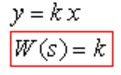
\includegraphics[scale = 0.5]{images/1_2.png}
		\end{minipage}
		&
		\begin{minipage}{.3\textwidth}
			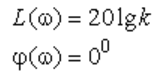
\includegraphics[scale = 0.5]{images/1_3_f.png}
		\end{minipage}
		\begin{minipage}{.3\textwidth}
			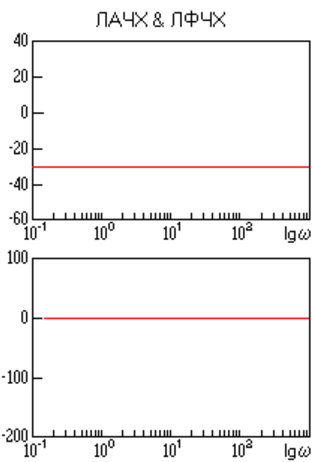
\includegraphics[scale = 0.5]{images/1_3.png}
		\end{minipage}
		&
		\begin{minipage}{.3\textwidth}
			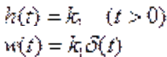
\includegraphics[scale = 0.5]{images/1_4.png}
		\end{minipage}
		&
		\begin{minipage}{.3\textwidth}
			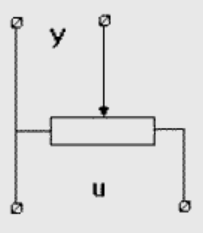
\includegraphics[scale = 0.5]{images/1_5.png}
		\end{minipage} \\ \hline
		
		Дифференцирующее звено
		&
		\begin{minipage}{.3\textwidth}
			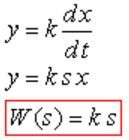
\includegraphics[scale = 0.5]{images/2_2.png}
		\end{minipage}
		&
		\begin{minipage}{.3\textwidth}
			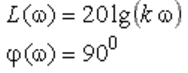
\includegraphics[scale = 0.5]{images/2_3_f.png}
		\end{minipage}
		\begin{minipage}{.3\textwidth}
			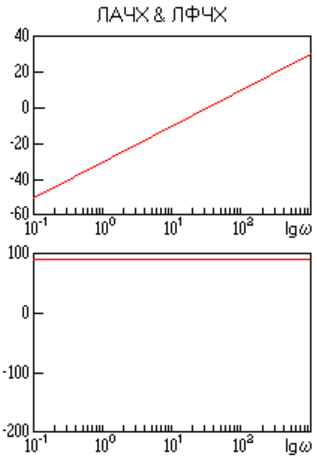
\includegraphics[scale = 0.5]{images/2_3.png}
		\end{minipage}
		&
		\begin{minipage}{.3\textwidth}
			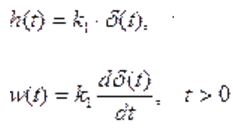
\includegraphics[scale = 0.4]{images/2_4.png}
		\end{minipage}
		&
		\begin{minipage}{.3\textwidth}
			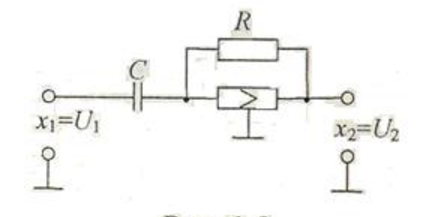
\includegraphics[scale = 0.3]{images/2_5.png}
		\end{minipage} \\ \hline
	\end{tabular}
	\egroup
\end{table}

\begin{table}[h!]
	\centering
	\bgroup
	\def\arraystretch{3}
	\begin{tabular}{ | m{3cm} | m{3.5cm} | m{4.5cm} | m{2.5cm} | m{2.5cm} }
		\hline
		Интегрирующее звено
		&
		\begin{minipage}{.3\textwidth}
			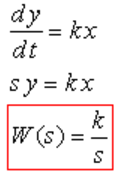
\includegraphics[scale = 0.5]{images/3_2.png}
		\end{minipage}
		&
		\begin{minipage}{.3\textwidth}
			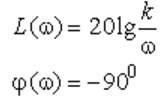
\includegraphics[scale = 0.5]{images/3_3_f.png}
		\end{minipage}
		\begin{minipage}{.3\textwidth}
			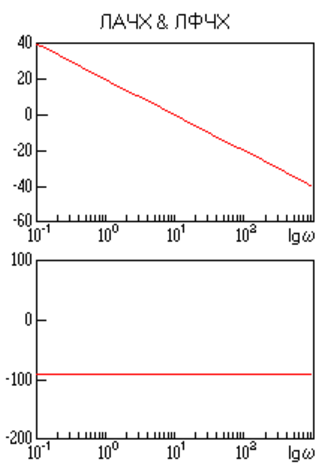
\includegraphics[scale = 0.5]{images/3_3.png}
		\end{minipage}
		&
		\begin{minipage}{.3\textwidth}
			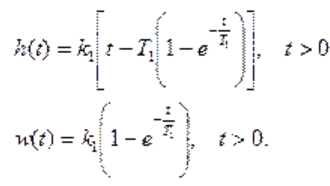
\includegraphics[scale = 0.3]{images/3_4.png}
		\end{minipage}
		&
		\begin{minipage}{.3\textwidth}
			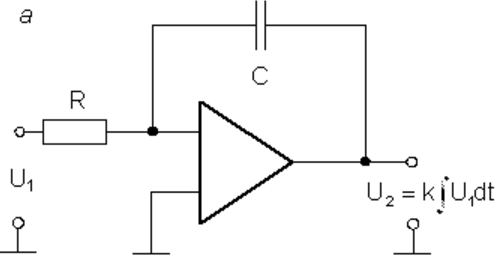
\includegraphics[scale = 0.2]{images/3_5.png}
		\end{minipage} \\ \hline
		
		Апериодическое звено первого порядка
		&
		\begin{minipage}{.3\textwidth}
			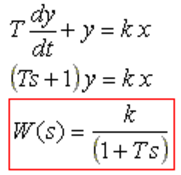
\includegraphics[scale = 0.5]{images/4_2.png}
		\end{minipage}
		&
		\begin{minipage}{.3\textwidth}
			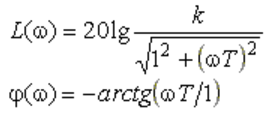
\includegraphics[scale = 0.5]{images/4_3_f.png}
		\end{minipage}
		\begin{minipage}{.3\textwidth}
			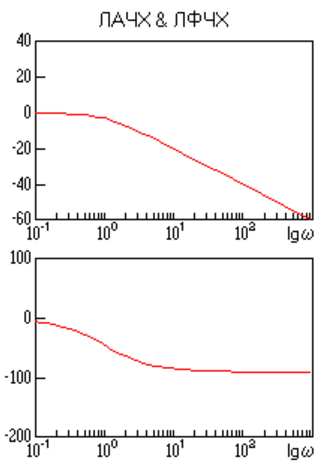
\includegraphics[scale = 0.5]{images/4_3.png}
		\end{minipage}
		&
		\begin{minipage}{.3\textwidth}
			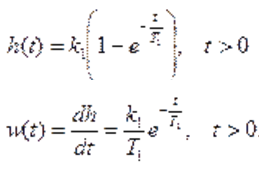
\includegraphics[scale = 0.35]{images/4_4.png}
		\end{minipage}
		&
		\begin{minipage}{.3\textwidth}
			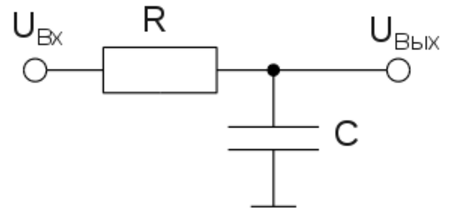
\includegraphics[scale = 0.2]{images/4_5.png}
		\end{minipage} \\ \hline	
		
		Форсирующее звено
		&
		\begin{minipage}{.3\textwidth}
			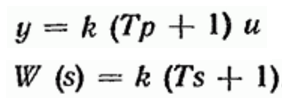
\includegraphics[scale = 0.45]{images/5_2.png}
		\end{minipage}
		&
		\begin{minipage}{.3\textwidth}
			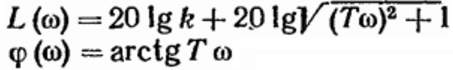
\includegraphics[scale = 0.35]{images/5_3_f.png}
		\end{minipage}
		\begin{minipage}{.3\textwidth}
			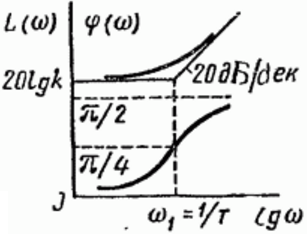
\includegraphics[scale = 0.5]{images/5_3.png}
		\end{minipage}
		&
		\begin{minipage}{.3\textwidth}
			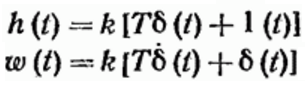
\includegraphics[scale = 0.32]{images/5_4.png}
		\end{minipage}
		&
		\begin{minipage}{.3\textwidth}
			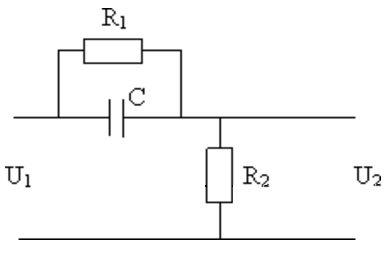
\includegraphics[scale = 0.22]{images/5_5.png}
		\end{minipage} \\ \hline
		
		Инерционно-дифференцирующее звено
		&
		\begin{minipage}{.3\textwidth}
			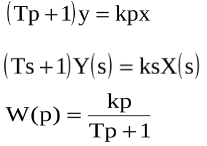
\includegraphics[scale = 0.5]{images/6_2.png}
		\end{minipage}
		&
		\begin{minipage}{.3\textwidth}
			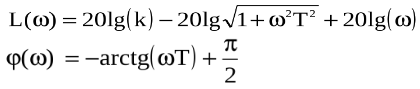
\includegraphics[scale = 0.4]{images/6_3_f.png}
		\end{minipage}
		\begin{minipage}{.3\textwidth}
			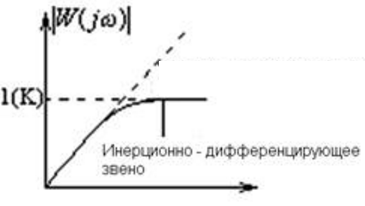
\includegraphics[scale = 0.5]{images/6_3.png}
		\end{minipage}
		&
		\begin{minipage}{.3\textwidth}
			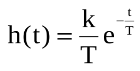
\includegraphics[scale = 0.4]{images/6_4.png}
		\end{minipage}
		&
		\begin{minipage}{.3\textwidth}
			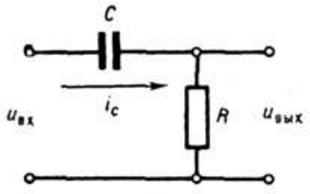
\includegraphics[scale = 0.32]{images/6_5.png}
		\end{minipage} \\ \hline	
	\end{tabular}
	\egroup
\end{table}

\begin{table}[h!]
	\centering
	\bgroup
	\def\arraystretch{4}
	\begin{tabular}{ | m{3cm} | m{3.5cm} | m{4.5cm} | m{2.5cm} | m{2.5cm} }		
		Изодромное звено
		&
		\begin{minipage}{.3\textwidth}
			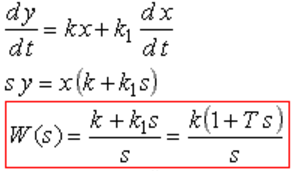
\includegraphics[scale = 0.4]{images/7_2.png}
		\end{minipage}
		&
		\begin{minipage}{.3\textwidth}
			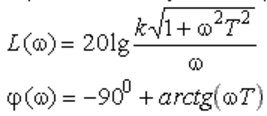
\includegraphics[scale = 0.5]{images/7_3_f.png}
		\end{minipage}
		\begin{minipage}{.3\textwidth}
			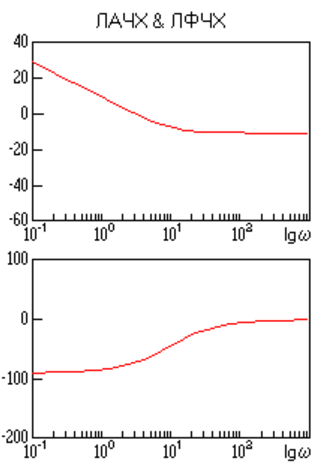
\includegraphics[scale = 0.5]{images/7_3.png}
		\end{minipage}
		&
		\begin{minipage}{.3\textwidth}
			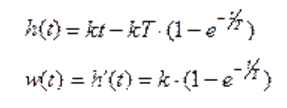
\includegraphics[scale = 0.34]{images/7_4.png}
		\end{minipage}
		&
		\begin{minipage}{.3\textwidth}
			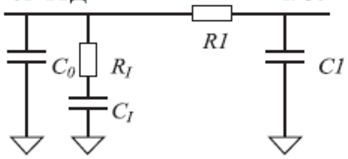
\includegraphics[scale = 0.27]{images/7_5.png}
		\end{minipage} \\ \hline
		
		Упругое звено
		&
		\begin{minipage}{.3\textwidth}
			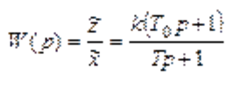
\includegraphics[scale = 0.5]{images/8_2.png}
		\end{minipage}
		&
		\begin{minipage}{.3\textwidth}
			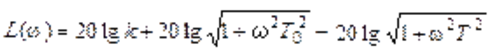
\includegraphics[scale = 0.35]{images/8_3_f.png}
		\end{minipage}
		&
		\begin{minipage}{.3\textwidth}
			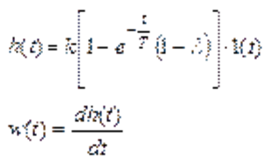
\includegraphics[scale = 0.35]{images/8_4.png}
		\end{minipage}
		&
		\begin{minipage}{.3\textwidth}
			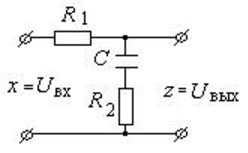
\includegraphics[scale = 0.40]{images/8_5.png}
		\end{minipage} \\ \hline
	\end{tabular}
	\egroup
\end{table}






\end{document}